\chapter{Test y resultados}\label{cap:test}

	En este capítulo se detallan las pruebas realizadas para verificar el correcto funcionamiento del sistema de actuación. Estas pruebas se han llevado a cabo en el banco de pruebas descrito en el capítulo \ref{cap:bancopruebas}, ya que es un entorno real y adecuado para probar el funcionamiento del actuador.

	Las pruebas están orientadas a verificar el funcionamiento del actuador y comprobar que es capaz de controlar la temperatura de la sala y ajustarla al valor óptimo. El intervalo de temperaturas usado para hacer las pruebas es [18{$^\circ$}C - 24{$^\circ$}C], ya que este intervalo garantiza un correcto funcionamiento de la sala. Para realizar las pruebas, no se ha utilizado el dato proporcionado por el algoritmo de optimización, sino que dicho valor está fijado de forma manual. El objetivo es comprobar que el sistema consigue fijar la temperatura de la sala al valor óptimo y comprobar que funciona correctamente. Una vez se compruebe su funcionamiento, se procederá a su integración en el sistema de optimización. 

	El sensor de la sala tiene una precisión de $\pm$ 0,5{$^\circ$}C, luego éste es el mínimo ajuste de temperatura que puede hacer el actuador. Por otro lado, hay que tener en cuenta que el actuador debe poder realizar ajustes de temperatura  pequeños  (de $\pm$ 0,5{$^\circ$}C o $\pm$ 1,0{$^\circ$}C) y grandes ($\pm$ 3{$^\circ$}C o superior). 

	Por tanto, para comprobar que el actuador es capaz de controlar la temperatura y realizar ajustes tanto pequeños como grandes, se han hecho 4 tipos de pruebas:

\begin{enumerate}
	\item Subir directamente la temperatura de la sala en al menos 3{$^\circ$}C.
           \item Bajar directamente la temperatura de la sala en al menos 3{$^\circ$}C.
           \item Subir la temperatura de la sala con incrementos de 0.5{$^\circ$}C.
           \item Bajar la temperatura de la sala con decrementos de 0.5{$^\circ$}C.
\end{enumerate} 

	Hay que aclarar que con estas pruebas se pretende verificar el funcionamiento en las situaciones más complejas. Se supone que si el sistema funciona correctamente en los casos extremos, también funcionará correctamente en los casos intermedios. A continuación se muestra la tabla \ref{tabla6_1:pruebas} con las caracteristicas de cada prueba realizada. 

	Por claridad, este capítulo sólo se incluye una prueba de cada tipo. En el anexo \ref{Anexo:experimentos} se incluyen otras pruebas realizadas para comprobar el funcionamiento del actuador. Las conclusiones obtenidas de todos los experimentos (incluidos los del anexo), se muestran en este capítulo.

\begin{table}[h]
\centering
\scalebox{0.80}[0.90]{
	\begin{tabular}{| c | c | c | c |}
		\hline
		\textbf{Num Exp} & \textbf{Tipo exp} &\textbf{Experimento}  & \textbf{Parámetros PID}\\
		\hline \hline
			\textbf{1} & 1 &Subida de 20{$^\circ$}C a 24{$^\circ$}C  & $K_{p}=28$ $K_{i}=0,037$  $ K_{d}=300$\\
		\hline
			\textbf{2} & 3 &Subida de 20{$^\circ$}C a 24{$^\circ$}en pasos de 0.5{$^\circ$}C & $K_{p}=28$ $K_{i}=0,037$  $ K_{d}=300$ \\
		\hline
			\textbf{3} & 2 & Bajada de 24{$^\circ$}C a 21{$^\circ$}C & $K_{p}=28$ $K_{i}=0,037$  $ K_{d}=300$\\
		\hline
			\textbf{4} & 4 &Bajada de 24{$^\circ$}C a 22{$^\circ$}C en pasos de 0.5{$^\circ$}C & $K_{p}=28$ $K_{i}=0,037$  $ K_{d}=300$\\
		\hline	
\end{tabular}}
\label{tabla6_1:pruebas}\caption{Características de los experimentos realizados}
 \end{table}

\section{Resultados de las pruebas}\label{sec:resultados}
A continuación se muestran unas capturas de \textit{Graphite} que muestran los resultados obtenidos de los 4 primeros experimentos. En cada captura se representa la temperatura a la que se encuentra la sala (azul), el \textit{setpoint} (verde), y la temperatura óptima (rojo).

\begin{figure}[htbp]
\centering
\textbf{Experimento 1}\\
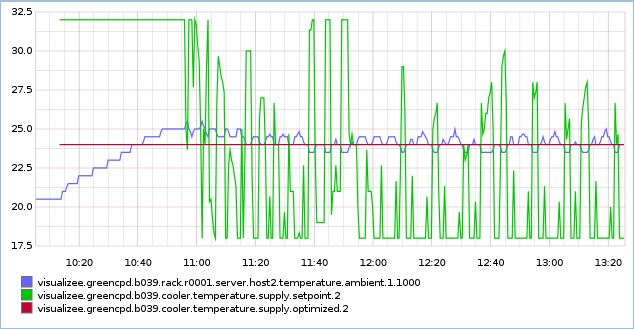
\includegraphics[width=120mm,height=85mm]{imagenes/capitulo6/experimento1}
\caption {Gráfica con los resultados del experimento 1}
\label{fig6_1:experimento1}
\end{figure}

\begin{figure}[htbp]
\centering
\textbf{Experimento 2}\\
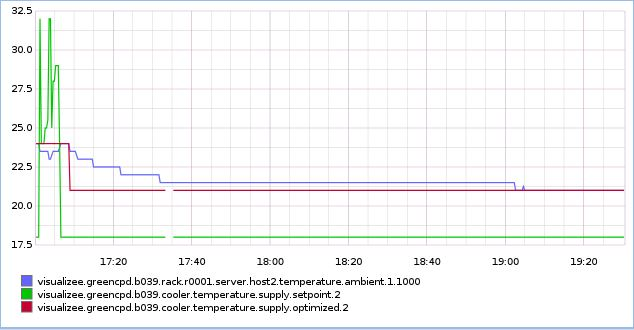
\includegraphics[width=120mm,height=85mm]{imagenes/capitulo6/experimento2}
\caption {Gráfica con los resultados del experimento 2}
\label{fig6_2:experimento2}
\end{figure}

\begin{figure}[htbp]
\centering
\textbf{Experimento 3}\\
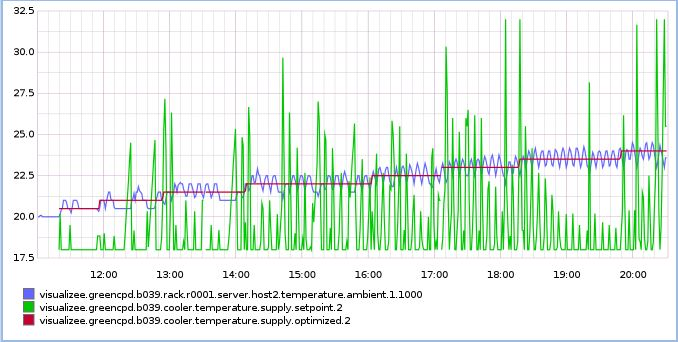
\includegraphics[width=120mm,height=85mm]{imagenes/capitulo6/experimento3}
\caption {Gráfica con los resultados del experimento 3}
\label{fig6_3:experimento3}
\end{figure}

\newpage

\begin{figure}[h]
\centering
\textbf{Experimento 4}\\
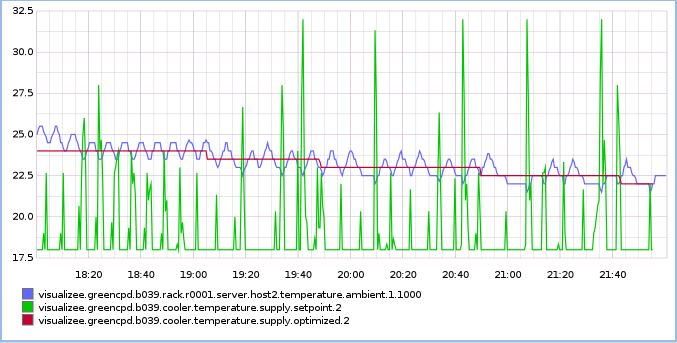
\includegraphics[width=120mm,height=85mm]{imagenes/capitulo6/experimento4}
\caption {Gráfica con los resultados del experimento 4}
\label{fig6_4:experimento4}
\end{figure}

	Hay que aclarar que en ninguna de las gráficas se ha incluido la señal de control. El motivo es que el controlador PID diseñado no tiene ningún mecanismo antiwindup, lo que hace que la señal de control en ocasiones tome valores demasiado grandes o pequeños que impiden visualizar correctamente el resto de señales. Se ha intentado añadir un mecanismo antiwindup al controlador pero no se han obtenido los resultados esperados. Por tanto, se ha decicido no incluir dicho mecanismo en este trabajo y se plantea la inclusión de este mecanismo como una linea futura. 

\section{Análisis de los resultados}\label{sec:análisis}
	Observando las gráficas de cada uno de los experimentos se comprueba que el actuador funciona correctamente y es capaz de controlar la temperatura del sistema y ajustarla al valor óptimo. Además, el actuador es capaz de ajustar la temperatura directamente o de forma gradual, lo que permite realizar ajustes de temperatura tanto pequeños como grandes. 

	 En todos los experimentos se observa un rizado en torno al valor óptimo. Este rizado es principalmente causado por la precisión del sensor. En principio, no supone un inconveniente a la hora de conseguir alcanzar la temperatura óptima, ya que suele ser pequeño y en la mayoría de las ocasiones coincide con la precisión del sensor.

	Hay que destacar el efecto windup que se ha producido en los experimentos 1, 5, 6, 8 y 11. El sistema de refrigeración dispone de un valor máximo y mínimo de funcionamiento y una vez que se alcanzan esos límites se satura. Sin embargo, el controlador PID diseñado es lineal por lo que el termino integral sigue aumentando y creciendo a pesar de que el sistema de refrigeración esté saturado. Cuando se supera la temperatura óptima, el error cambia de signo y el término integral comienza a compensarse aunque tardará un cierto tiempo como consecuencia del error acumulado en la etapa de subida. Esto provoca que se produzca una sobreoscilación, como se observa al inicio de los experimentos mencionados. 

	Este efecto es habitual que ocurra cuando se produce variaciones muy grandes de temperatura que se aproximan a la longitud del intervalo. Esta situación es poco probable que ocurra en un CPD, ya que es más habitual que el ajuste de temperatura sea gradual que ir moviéndose de extremo a extremo. A pesar de este efecto, se observa que el sobreajuste no es muy elevado y en poco tiempo la temperatura se estabiliza en torno a su valor óptimo.  Como ya se ha comentado, una posible mejora de este trabajo sería la implementación de un controlador PID con mecanismo antiwindup para corregir este problema.

	También se puede observar cómo influye la temperatura del exterior en la sala. En los experimento 2 y 7 se observa que la temperatura decae rápidamente pero a partir de un cierto valor, la temperatura tarda más tiempo en disminuir. Este efecto es provocado debido a la influencia de la temperatura exterior. El ciclo de evaporación se realiza en el exterior del edificio y si la temperatura exterior es elevada la eficiencia del ciclo de refrigeración se reduce y esto hace que tarde más tiempo en bajar la temperatura de la sala. Además, hay que recordar que el sistema de refrigeración del banco de pruebas es un aire acondicionado doméstico que no está diseñado para este tipo de salas, por lo que existe una limitación física que es ajena al sistema de actuación. Este efecto también se produce durante el invierno aunque de forma inversa. Esta es una de las razones por la que no se ha podido comprobar el funcionamiento del actuador en el caso de subir y bajar la temperatura de extremo a extremo.










